%% This Beamer template is based on the one found here: https://github.com/sanhacheong/stanford-beamer-presentation, and edited to be used for Stanford ARM Lab

\documentclass[10pt]{beamer}
%\mode<presentation>{}

\usepackage[spanish]{babel}
\usepackage{media9}
\usepackage{amssymb,amsmath,amsthm,enumerate}
\usepackage[utf8]{inputenc}
\usepackage[T1]{fontenc}
\usepackage{array}
\usepackage[parfill]{parskip}
\usepackage{graphicx}
\usepackage{caption}
\usepackage{subcaption}
\usepackage{bm}
\usepackage{amsfonts,amscd}
\usepackage[]{units}
\usepackage{listings}
\usepackage{multicol}
\usepackage{multirow}
\usepackage{tcolorbox}
\usepackage{physics}
\usepackage{circuitikz}

% Enable colored hyperlinks
%\hypersetup{colorlinks=true}

% The following three lines are for crossmarks & checkmarks
\usepackage{pifont}% http://ctan.org/pkg/pifont
\newcommand{\cmark}{\ding{51}}%
\newcommand{\xmark}{\ding{55}}%

% Numbered captions of tables, pictures, etc.
\setbeamertemplate{caption}[numbered]

%\usepackage[superscript,biblabel]{cite}
\usepackage{algorithm2e}
\renewcommand{\thealgocf}{}

% Bibliography settings
\usepackage[style=ieee]{biblatex}
\setbeamertemplate{bibliography item}{\insertbiblabel}
\addbibresource{references.bib}

% Glossary entries
\usepackage[acronym]{glossaries}
\newacronym{ML}{ML}{machine learning}
\newacronym{HRI}{HRI}{human-robot interactions}
\newacronym{RNN}{RNN}{Recurrent Neural Network}
\newacronym{LSTM}{LSTM}{Long Short-Term Memory}


\theoremstyle{remark}
\newtheorem*{remark}{Remark}
\theoremstyle{definition}

\newcommand{\empy}[1]{{\color{darkorange}\emph{#1}}}
\newcommand{\empr}[1]{{\color{cardinalblue}\emph{#1}}}
\newcommand{\examplebox}[2]{
\begin{tcolorbox}[colframe=darkcardinal,colback=boxgray,title=#1]
#2
\end{tcolorbox}}

\usetheme{Stanford} 
\def \i  {\item}
\def \ai {\item[] \quad \arrowbullet}
\newcommand \si[1]{\item[] \quad \bulletcolor{#1}}
\def \wi {\item[] \quad $\ \phantom{\Rightarrow}\ $}
\def \bi {\begin{itemize}\item}
\def \ei {\end{itemize}}
\def \be {\begin{equation*}}
\def \ee {\end{equation*}}
\def \bie {$\displaystyle{}
\def \eie {{\ }$}}
\def \bsie {\small$\displaystyle{}
\def \esie {{\ }$}\normalsize\selectfont}
\def \bse {\small\begin{equation*}}
\def \ese {\end{equation*}\normalsize}
\def \bfe {\footnotesize\begin{equation*}}
\def \efe {\end{equation*}\normalsize}
\renewcommand \le[1] {\\ \medskip \lefteqn{\hspace{1cm}#1} \medskip}
\def \bex {\begin{example}}
\def \eex {\end{example}}
\def \bfig {\begin{figure}}
\def \efig {\end{figure}}
\def \btheo {\begin{theorem}}
\def \etheo {\end{theorem}}
\def \bc {\begin{columns}}
\def \ec {\end{columns}}
\def \btab {\begin{tabbing}}
\def \etab {\end{tabbing}\svneg\svneg}
\newcommand \col[1]{\column{#1\linewidth}}
\def\vneg  {\vspace{-5mm}}
\def\lvneg {\vspace{-10mm}}
\def\svneg {\vspace{-2mm}}
\def\tvneg {\vspace{-1mm}}
\def\vpos  {\vspace{5mm}}
\def\lvpos {\vspace{10mm}}
\def\svpos {\vspace{2mm}}
\def\tvpos {\vspace{1mm}}
\def\hneg  {\hspace{-5mm}}
\def\lhneg {\hspace{-10mm}}
\def\shneg {\hspace{-2mm}}
\def\thneg {\hspace{-1mm}}
\def\hpos  {\hspace{5mm}}
\def\lhpos {\hspace{10mm}}
\def\shpos {\hspace{2mm}}


% commands to relax beamer and subfig conflicts
% see here: https://tex.stackexchange.com/questions/426088/texlive-pretest-2018-beamer-and-subfig-collide
\makeatletter
\let\@@magyar@captionfix\relax
\makeatother

\title[Proyecto Final]{Estudio e implementación de un administrador de baterías de Litio-ion}
\subtitle{Presentación de Avances}

%\beamertemplatenavigationsymbolsempty

\begin{document}

\institute{
	\vskip 5pt
	\begin{figure}
		\centering
		\begin{subfigure}[t]{0.5\textwidth}
			\centering
			
\includegraphics[height=0.7in]{./images/LOGO-UNR-NEGRO.png}
		\end{subfigure}%
		~ 
		\begin{subfigure}[t]{0.5\textwidth}
			\centering
			
\includegraphics[height=0.5in]{./images/FCEIA-logo.png}
		\end{subfigure}
	\end{figure}
	\vskip 5pt
	Facultad de Ciencias Exactas, Ingeniería y Agrimensura\\
	Universidad Nacional de Rosario\\
	\vskip 1pt
}

\author[Escuela de Ingeniería Electrónica]{
	\begin{tabular}{ccc} 
	Federico Ceccarelli & Martin Moya & Lucio Santos\\
    \footnotesize
	\texttt{\href{mailto:fededc88@gmail.com}{fededc88@gmail.com}} &
	\footnotesize
	\texttt{\href{mailto:moyamartin1@gmail.com}{moyamartin1@gmail.com}} &
  	\footnotesize
	\texttt{\href{mailto:lucio.santos2206@gmail.com}{lucio.santos2206@gmail.com}}
\end{tabular}
\vspace{-4ex}}



\date{\today}

\begin{noheadline}
\begin{frame}\maketitle\end{frame}
\end{noheadline}

\setbeamertemplate{itemize items}[default]
\setbeamertemplate{itemize subitem}[circle]

\begin{frame}
	\frametitle{Contenidos} % Table of contents slide, comment this block out to remove it
	\tableofcontents % Throughout your presentation, if you choose to use \section{} and \subsection{} commands, these will automatically be printed on this slide as an overview of your presentation
\end{frame}

\section{Avances}
% `[allowframebreaks]` can be used to have multiple slides in one frame, where the slides are continued with the suffix "(cont.)"; `[allowframebreaks]` can be used with `\framebreak` to manually break each frame into multiple slides
\begin{frame}[allowframebreaks]
\frametitle{Avances del Proyecto}
	\begin{itemize}
	  \item Selección del Sensor de corriente
	  \item Diseño de un modelo de una celda de Litio-Ion
	  \item Estimación del estado de carga utilizando un Filtro de Kalman
	\end{itemize}
\end{frame}

\section{Sensor de Corriente}

\begin{frame}[allowframebreaks]
	\frametitle{Objetivos}
	Medir la corriente que circula por el pack de baterías nos permite:
	\begin{itemize}
	  \item Mantener al pack operando dentro del SOA.
	  \item Monitorear la distribución de carga entre celdas
	  \item Implementar y mantener un seguimiento preciso del SoC
	\end{itemize}
\end{frame}

\begin{frame}[allowframebreaks]
\frametitle{Tecnologías disponibles}
	\begin{itemize}
	  \item \textbf{Resistencia Shunt}
	  \item Transformador de Intensidad
	  \item \textbf{Sensor de Efecto Hall}
	  \item Sensor de Impedancia Magnética
	  \item Sensor de Magnetoresistencia Gigante
	  \item Sensores Ópticos
	\end{itemize}
\end{frame}


\begin{frame}[allowframebreaks]
	\frametitle{Resistencia Shunt}
	Calcula la corriente de forma indirecta midiendo la caída de tensión sobre
	una resistencia, que tiene un valor del órden de los miliohmios, al circular
	la corriente incógnita, su esquemático se puede observar en la Figura
	\ref{sch_shunt}.

	\begin{figure}[h!]
	  \begin{circuitikz}\draw
		(0, 0) to[resistor, i_>=$I$] (6, 0)
		;
		\draw
		(2, 0) to[short, *-] (2, 1)
		(2, 1) to[voltmeter] (4, 1)
		(4, 1) to[short, -*] (4, 0)
		;
	  \end{circuitikz}
	  \caption{Esquemático de un sensor de corriente por resistencia shunt}
	  \label{sch_shunt}
	\end{figure}

\end{frame}
% This demonstrates a new section
\section{Examples}
% This demonstrates a single frame without framebreaks
\begin{frame}{Example of Horizontal Subfigures}

	\begin{figure}
		\centering
		\begin{subfigure}[t]{0.5\textwidth}
			\centering
			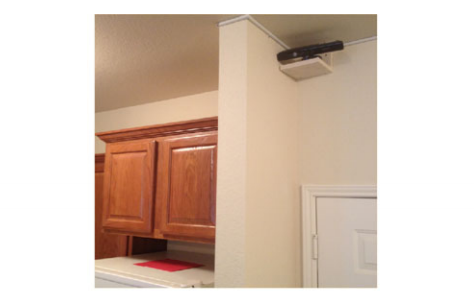
\includegraphics[width=0.9\textwidth]{images/stone2014fall_setup.png}
			\caption{Single Kinect setup for fall prevention in elderly residence \cite{stone2014fall}}
		\end{subfigure}%
		~ 
		\begin{subfigure}[t]{0.5\textwidth}
			\centering
			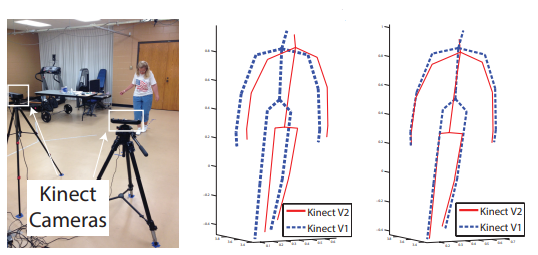
\includegraphics[width=\textwidth]{images/staranowicz2015easy_multiple_kinects.png}
			\caption{Multiple Kinects calibration for fall prediction\cite{staranowicz2015easy}}
		\end{subfigure}
		\caption{Examples of Horizontal Subfigures}
	\end{figure}
\end{frame}

\begin{frame}{Example of Horizontal Alignment}
    % For data collection:
    
    Example of Horizontal Alignment of a \texttt{table} and a \texttt{figure}.
    \begin{center}
    \begin{minipage}[t]{.65\linewidth}
    \begin{table}[H]
    % \renewcommand{\arraystretch}{1.3}
    \caption{Environment limitations on data collection}
    \label{tab:env_limit}
    \centering
    % \begin{tabular}{m{1.6cm}|c|>{\centering\arraybackslash}m{2cm}|>{\centering\arraybackslash}m{2.3cm}}
    \begin{tabular}{m{2cm}|c|c|>{\centering\arraybackslash}m{1.5cm}}
    % \begin{tabular}{c|c|c|c}
        & Kinect & Stereo & Kinect + Stereo\\
        \hline
        Indoor & \cmark & \cmark & \cmark \\
        \hline
        Outdoor & \xmark & \cmark & \cmark \\
        \hline
        High number of features & \cmark & \cmark & \cmark \\
        \hline
        Low number of features & \cmark & \xmark & \cmark 
    \end{tabular}
    \end{table}
    \end{minipage}%
    \begin{minipage}[t]{.35\linewidth}
    \vspace{0pt}
    \centering
    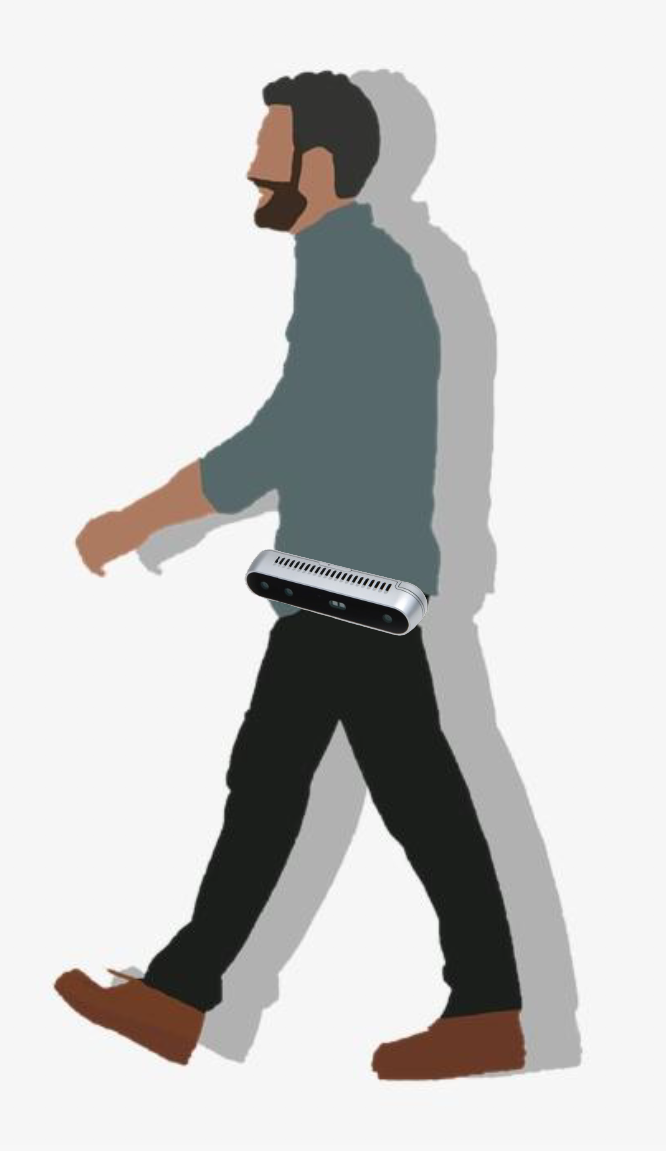
\includegraphics[width=0.7\textwidth]{images/waist_cam_setup_new.png}
    \end{minipage}
    \end{center}
\end{frame}

\begin{frame}[allowframebreaks]
\frametitle{Example of resizable equations}

\begin{center}
\scalebox{1.0}{\parbox{\linewidth}{%
		\begin{align*}
		& {\text{min \hskip 6pt}}
		& & J = \int (a_{real} - \hat{a})^2  \\
		& \text{subject to}
		& & \text{human kinematics} \\
		&&& \text{no collision} \\
		&&& \text{no falling} 
		\end{align*}
}}
\end{center}
\end{frame}

\begin{frame}[allowframebreaks]
\frametitle{Example of Regular Equations}
    % \begin{equation}
    %     {}^Ag = {}^AR_B {}^Bg
    % \end{equation}
    
    % \begin{equation}
    %     V = \frac{{}^Bg \cross {}^Ag}{\norm{{}^Ag}\norm{{}^Bg}}, 
    %     \theta = \arccos{\frac{{}^Bg \cross {}^Ag}{\norm{{}^Ag}\norm{{}^Bg}}}
    % \end{equation}
    
    \begin{equation}
        \begin{split}
        {}^AR_{B}(t_0)=\left[\begin{array}{ccc}
        1 & 0 & 0 \\
        0 & 1 & 0 \\
        0 & 0 & 0
        \end{array}\right]+
        \sin (\theta)\left[\begin{array}{ccc}
        0 & -v_{3} & v_{2} \\
        v_{3} & 0 & -y_{1} \\
        -v_{2} & v_{1} & 0
        \end{array}\right]+ \\
        (1-\cos (\theta))\left[\begin{array}{ccc}
        0 & -v_{3} & v_{2} \\
        v_{3} & 0 & -v_{1} \\
        -v_{2} & v_{1} & 0
        \end{array}\right]^{2}
        \end{split}
        \end{equation}
        
        \begin{align}
            {}^AR_{B}(t) &= \Delta R {}^AR_{B}(t_0) \\
            \Delta R &= {}^AR_{B}(t) {}^AR_{B}^T(t_0)
        \end{align}
\end{frame}

\begin{frame}[allowframebreaks]
\frametitle{Example of Video}

	\includemedia[
	width=\linewidth,
	totalheight=0.6\linewidth,
	activate=pageopen,
	passcontext,  %show VPlayer's right-click menu
	addresource=images/opensim_video.mp4,
	flashvars={
		%important: same path as in `addresource'
		source=images/opensim_video.mp4
	}
	]{\fbox{Click!}}{VPlayer.swf}
    
\end{frame}

\begin{frame}[allowframebreaks]
\frametitle{Bibliography}
\printbibliography
\end{frame}

\end{document}
